\chapter{Industry Application Scenarios}

Bitcoin is an emergent phenomenon realized through the subtle interaction of multiple data structures and incentive mechanisms. 
In isolation the various components that comprise the Bitcoin protocol are well known and in some cases have existed for years.
The novelty of Bitcoin was to combine these elements in a previously unimagined way. 
The success of Bitcoin as a cryptocurrency has generated interest in the design principles employed to realize the system.
This in turn has prompted some to critically reassess traditional methods used to process information. 
The purpose being to determine the extent to which architectural aspects of Bitcoin might be replicated in analogous scenarios to reduce or eliminate current inefficiencies. 

\section{Supply-Chain} 

The concept of blockchain, as described by Figure 1.2, is only one aspect of the Bitcoin mechanics that present compelling properties to enterprise information technology engineers.
In this section we describe a small subset of the properties that facilitate useful industry application, especially in the service of supply chain management systems. 

\subsection*{Related Work} 

There are two ``smart contract'' based projects attempting to realize the goal of ameliorating supply chain management through the development of a ``blockchain'' data structure. 
One such operation, known as Provenance states explicitly in the first paragraph of their technical whitepaper ``\textit{the Decentralized Application (Dapp) proposed in this paper is still in development}''.
Another organization under the name of Skuchain does not exhibit a dedicated technical whitepaper describing how their proposed system would work. 
Distinct from these \textit{high level ideas} of how ``blockchain'' technology could be applied towards the improvement of supply chain management, in this section we detail several concrete recommendations. 

\subsection{Data-Structures \& Design Principles}

We highlight a number of fundamental design principles, and where relevant their associated data-structures or cryptographic properties, present in the design of Bitcoin and propose a mapping for how these aspects might be usefully employed in the design of an operational supply chain management system. 

\begin{figure}
  \centering
    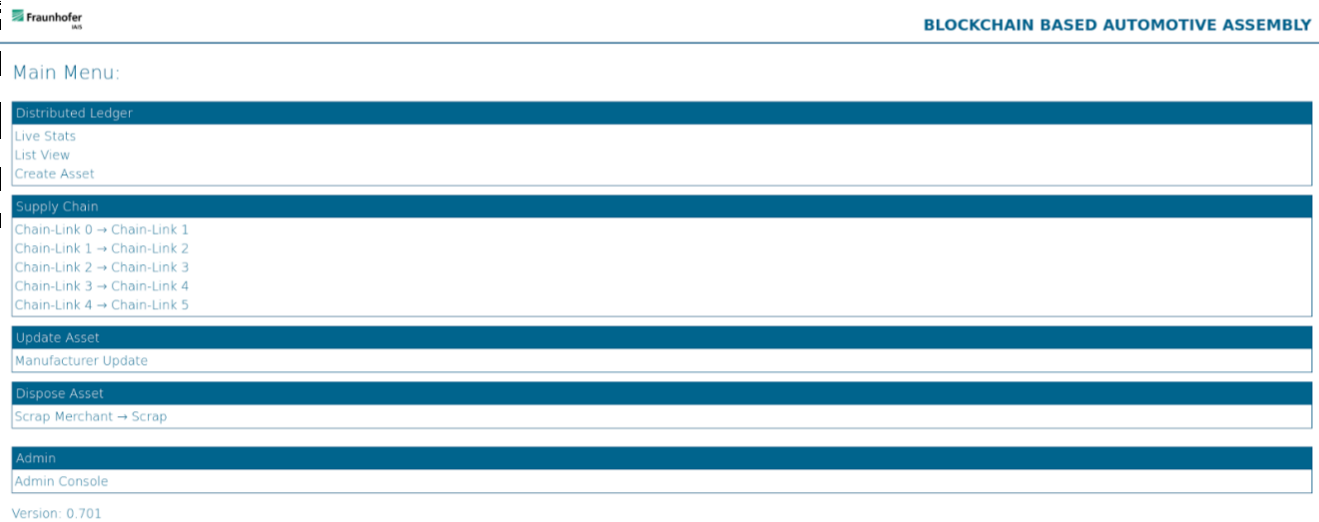
\includegraphics[width=0.8\textwidth]{go0}
  \caption{Main Administrator Dashboard}
\end{figure}

\subsubsection{Pseudo-Anonymity}

This characteristic is one of the fundamental tenants of the ``cypherpunk'' movement that gave rise to the concept of cryptocurency.
Furthermore, practical fungability of individual Bitcoins is important to the viability of this technology as a medium of exchange. 
Association with nefarious activity such as coins that have been involved in deep web market drug deals, such as those that regularly take place on AlphaBay Market, would be subject to confiscation by authorities were they to be positively identified. 
What makes cryptocurrencies attractive to these users in the first place is the property of pseudo-anonymity. 
Network participants are represented only by their address, which if used in accordance with best security practices can be very difficult to associate with a real-world identity. 

These practices employed by $21^{st}$ century drug dealers stand in stark contrast to the techniques employeed in the 1980's, such as those demonstrated in the 2001 movie Blow.
This film also serves to portray a critical aspect of supply chains. 
When the American cocaine importer George Jung introduces his ``Columbian connection'', Diego Delgado, to the head of his distribution network Derek Foreal they are quick to extricate Jung from the process, to his great dismay. 
This brief anecdote serves to underscore the importance of supply chain nodes not being able to identify nodes to whom they are not directly connected, lest they use that resource to ``cut out'' the middleman. 
Representing nodes in a supply chain in such a way that we are able to trace the goods they move through the network while preventing them from de-anonymizing one another is a critical component to a functional supply chain system. 
The pseudo-anamity properties of the Bitcoin network can be usefully applied to the creation of a shared data structure with these constraints. 

% https://en.wikipedia.org/wiki/Replication_(computing)
\subsubsection{Replicated Database}

The idea of using a replicated database to prevent against the corruption of information resources is a well-worn advantageous approach. 
Replication in computing involves sharing information so as to ensure consistency between redundant resources, such as software or hardware components, to improve reliability, fault-tolerance, or accessibility.
Recently this approach has been employed with success by the ``big data'' framework Apache Hadoop among others. 
Bitcoin likewise utilizes this approach by storing a full copy of the blockchain on each network node. 
In a supply chain management system infused with elements inspired by the Bitcoin design the inclusion of the data replication paradigm is important to ensuring that all stakeholders can maintain and independently verify their own copy of the flow of goods or merchandise components. 

\begin{figure}
  \centering
    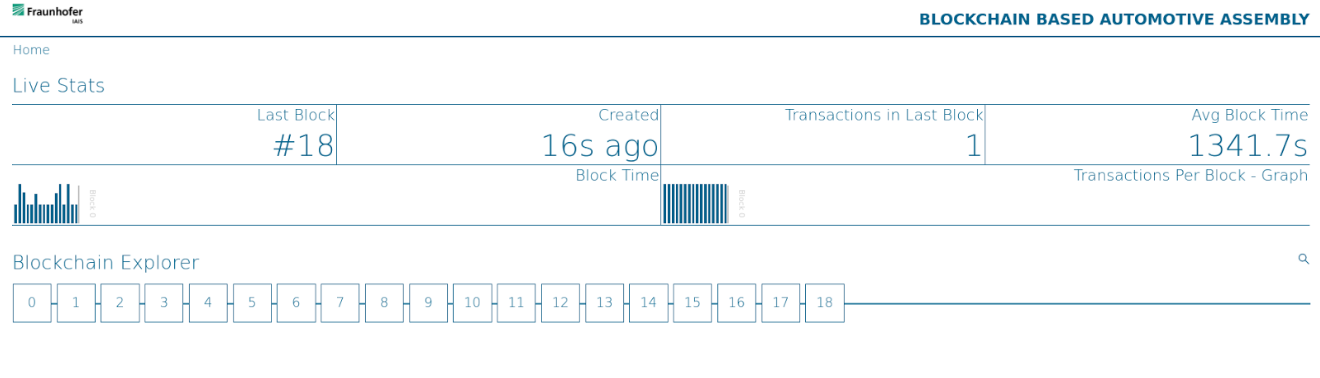
\includegraphics[width=0.8\textwidth]{go1}
  \caption{Blockchain Data Exploration Terminal}
\end{figure}

\subsubsection{Distributed Consensus}

This is a concept closely related to the above section. 
The consensus model in the simplest sense would operate as a mutual agreement between contracting parties and it would take signed acknowledgement of both parties to certify a transaction (or perhaps some other ``proof-of-work'').
Ensuring that the replicated data-sets in each node can form an agreement on a common history.
This process allows different organizations with competing interests to agree on a consistent record.

\subsubsection{Provenance of Data}

To spend a Bitcoin requires that its provenance be explicitly verified against the entire transaction history of the network. 
This feature is beneficial to supply chain systems concerned with targeted recall of defective products, especially so since each individual Bitcoin exists as a unit within the system and cannot be merely \texttt{Crtl + v, Ctrl + v}'d into existence, enforcing uniqueness. 

Targeted recall of products effected by particular components is an important concern to many organizations, for instance large automotive manufacturers. 
In 2015 the Volkswagen emissions scandal (VW-Abgasaff{\"a}re) prompted a vast recall campaign of large subsets of vehicles. 
The problem of tracking vehicle components through the inherent ``mixing'' process that goes on through a supply chain, from material aggregation to finished production is analogous to tracking ``tainted'' coins through the Bitcoin network. 

\subsubsection{Proof-of-Work}

The Bitcoin proof-of-work exhausts computation resources, and ultimately electricity (among other considerations, i.e. the raw materials used to fashion hardware components) in the expending of a scare resource, the money used to buy it, in order to bring new Bitcoins into existence. 
There are alternative models to proof-of-work, one of which is proof-of-stake, even CAPTCHAs could be thought of as a kind of proof-of-work spending, typically, the limited resource of advanced (ideally human-level) visual processing skills. 
Another scarce resource is reputation.
The envisaged system would employ this resource through the reputation associated with an individual private key signature, for a transaction to be committed it would necessitate a signature by both transaction parties, i.e. the transaction quorum. 

\subsubsection{Threat model}

Counterfeiting is a problem that many brands are worried about.
Disingenuous goods circulate widely on the web, and initiatives such as \texttt{code.moncler.com} by French luxury goods manufacturer Moncler which tries to encourage users to register the QR stitched into their product are attempting to combat this growing trend. 
Such as system as we propose here would assist in the tracking of provenance for all goods. 

Another potential threat is that of simple data-corruption, loss, or human-input error. 
The distributed nature of the data model, together with a pre-arranged ``consensus threshold'' or mutual agreement could serve as a resolution to this issue. 
Thereby we prevent corruption of data by malicious parties or equipment malfunction.


\begin{figure}
  \centering
    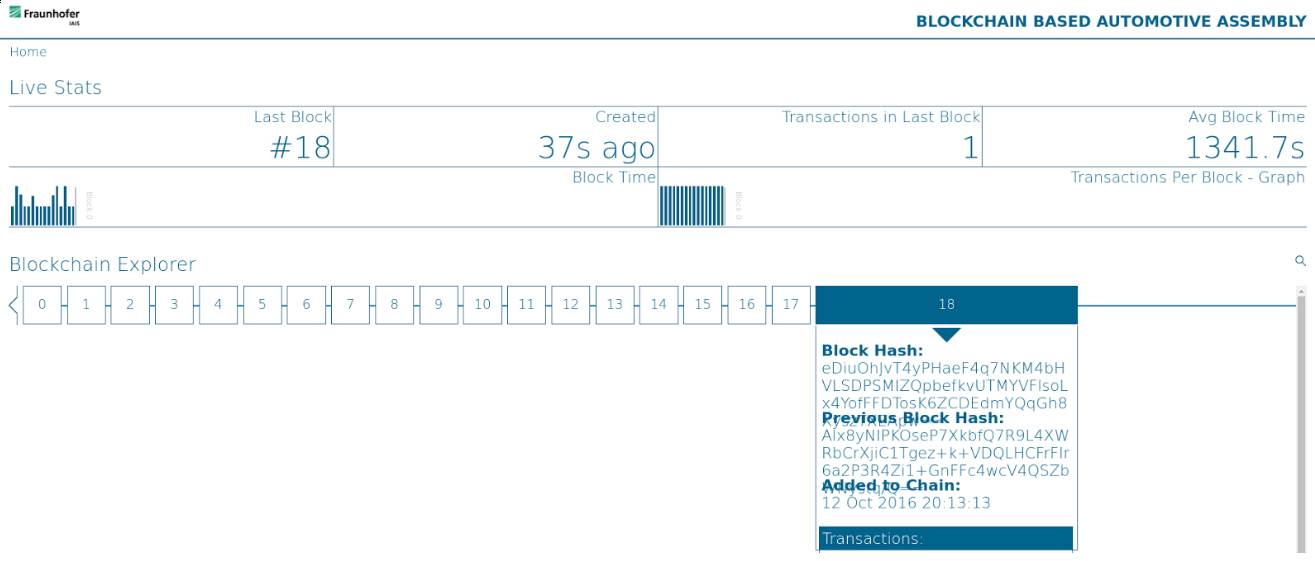
\includegraphics[width=0.9\textwidth]{go2}
  \caption{Transaction Drill-Down}
\end{figure}

\subsubsection{Consortial Blockchain}

This system would be public only among interested parties.
It would spread out emanating from the individual quora of users and gradually could be made extensible to incorporate different components of the network.

\subsection{Demo}

The design framework described in this section was partially realized as an entry in the Hyperledger Blockchain Hackathon of October $3^{rd}$ in Amsterdam for which it was awarded the grand prize in the category of ``outside team''\footnote{http://hollandfintech.com/winner-hyperledger-blockchain-hackathon-announced/}. 


\subsubsection{Discussion}

In \cite{narayanan2016bitcoin} it is pointed out that Satoshi was probably not an academic because he implemented his system first and then wrote about it later, and academics tend to do the opposite. 
This work proves the accuracy of that assertion.
The supply chain management protocol herein described remains to be implemented in code, what this work attempts to do is clearly specify the design of properties that such a system would seek to achieve. 

\begin{figure}
  \centering
    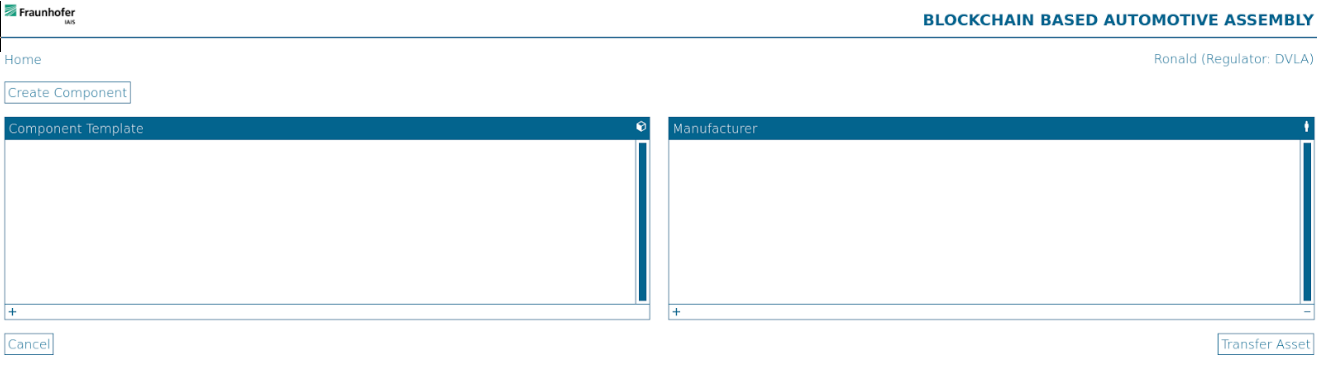
\includegraphics[width=0.9\textwidth]{go3}
  \caption{Primary User Interface Scenario}
\end{figure}
 
\subsection*{Remarks}

In assessing the merits of a technology one is never fully correct and incorrect to prefer one method over another. 
In creating this chapter I might have individually type-set each letter, printed it with ink, and scanned the result into my computer, I chose the more difficult route and used \LaTeX.
Which method is more similar to the use of the designs described above to the complex issues faced in today's long and convoluted supply chains? 
The final determination of the degree to which these techniques are practically useful in the supply chain process is empirical. 
This rough framework and design methodology remains to be validated but nevertheless it is the result of careful consideration on the process whereby one might derive concrete value through the actionable properties of the Bitcoin protocol melded with the real-world problems of a supply chain. 

%%%%%%%%%


% Pseudo-Anonymity

% One of the fundamental tenants of the ``cypherpunk'' movement that gave rise to the concept of cryptocurency

% Fungability remains a primary concern of the Bitcoin core dev community

% Indispensable characteristic of supply chains


% Replicated Database

% In Bitcoin all full nodes retain a complete copy of the database 
% Principle demonstrated to be effective by protocols such as MapReduce 
% Prevents corruption of data by malicious parties or equipment malfunction

% Provenance of Data

% To spend a Bitcoin requires that its provenance be explicitly verified against the entire transaction history of the network 
% Potential benefit to supply chain systems concerned with targeted recall of defective products

% Distributed Consensus

% Ensuring that the replicated datasets in each node can form an agreement on a common history 
% Allows different organizations with competing interests to agree on a consistent record

% Proof of Work

% CAPTCHA 
% Adam Back’s hashcash 
% Proof of stake 
% Private key signatures

% The data structure that supports the cryptocurrency Bitcoin
% Market Cap: \$10,107,045,577 
% Years Operational: 7 
% Number of Addresses: 1.9 million 
% Arguably the world’s only functional blockchain application

% Designing a Data Structure with Properties Similar to Bitcoin’s Data Structure
% Bitcoin and Cryptocurrency Technologies Arvind Narayanan
% “Private blockchain” is just a confusing name for a shared database

\section{Real Estate Property Rights}

Across the Third World, from Honduras to the Republic of Georgia, efforts are underway to establish land titles via the Blockchain. Proponents of this system advocate it as a mechanism to enable marginalized residents of the world's slums to take out loans using this newly recognized property as collateral.

The commodification of people's homes for use as financial instruments was at the heart of the financial crisis of 2008. The correlation between those toxic assets and the Blockchain-based property schemes which are now in the early phases of implementation warrant close scrutiny. Failing to learn the lessons of the last financial meltdown may precipitate another massive disenfranchisement of the world's most vulnerable citizens.

\subsection*{Land Grab Mania}

The financial crisis of 2008 is considered by many economists to have been the worst since the Great Depression of the 1930s. The impetus of this man-made disaster was the securitization of home mortgages which were subsequently arranged into tranches and partitioned on the basis of repayment expectation.

Predatory lenders issued mortgages to unsuspecting victims in the form of NINJA loans (No Income No Job or Assets). These financial instruments were thrust upon people with no real hope of paying them back and the result was countless families losing their homes when the system imploded in 2008.

Hernando de Soto is President of the Institute for Liberty and Democracy. De Soto espouses the notion that residents of Third World shanties such as the Juhu slums of Mumbai, depicted in the film Slumdog Millionaire, are essentially locked out of global capital markets by their inability to secure credit.

\subsection*{Slum property rights}

Officially such people are homeless, lacking governmental title to their domicile. However, the facts on the ground tell a different story. Typically members of these local communities are conscious of one another's de facto property rights, which are acknowledged and respected.

Prior efforts to establish title to such slum properties have resulted in failure as corrupt officials allocated land rights on the basis of favoritism or influence. The Semantic Blockchain presents an appealing alternative as the consensus mechanism might ensure that a majority of residents would act in good faith and correctly assign addresses.

``Of the 7.3 billion people in the world, only 2 billion have a title that is legal, effective and public regarding their control over an asset''. remarked De Soto in a public statement. 
``When something is not legally on record as being owned, it can therefore not be used... as collateral to get credit, as a credential that you can be able to transfer part of your property to invite investment in. Things are owned, but when they're not adequately paperized or recorded, they cannot fill the functions of creating capital and credit''.

\subsection*{Toxic Assets in the Making}

A collateralized debt obligation (CDO) is a type of structured asset-backed security (ABS). 
Originally developed for the corporate debt markets, over time CDOs evolved to encompass the mortgage and mortgage-backed security (MBS) markets. 
In the years leading up to the crash of 2008 some MBS issuers, such as Fannie Mae and Freddie Mac, guaranteed against homeowner default risk while requiring private mortgage insurance on loans in which the borrower provided a down payment of less than 20\% of the property value.

\subsection*{Decentralized insurance}

Together these financial instruments comprised the toxic assets that necessitated the infamous government bailouts which may have been a motivation behind the creation of the world's first digital currency.
Recall that the genesis block of Bitcoin in fact time-stamped itself using the text \textit{The Times 03/Jan/2009 Chancellor on brink of second bailout for banks}.

Peer-to-peer, decentralized, and even autonomous insurance is a concept which is recently gaining traction in the Blockchain community. 
The London Fintech Week Blockchain Hackathon generated a smart contract insurance system which would provide instant compensation on a variety of claims.

In light of pilot projects taking aim at a Blockchain-based land registry currently under way it appears as if a network of mortgage-backed securities generated by first-time borrowers in the Third World might be a near term reality.

It is conceivable that these insurance contracts could, in the foreseeable future, be combined with autonomous smart contract mechanisms to create a DAO (decentralized autonomous organization) of MBS. This has the potential to usher in a new wave of financialization of people's homes.

\subsection*{Learn the lesson of DAO disaster}

Under such a regime repayment tranches could be configured and rated automatically providing more transparency in an industry notoriously opaque to customers and regulators alike.

Lest we fall prey to an epidemic of irrational exuberance we might do well to remember the recent disaster of the DAO and temper our excitement. A system such as the one herein described could unlock vast economic potential, or, to paraphrase Michael Lewis, it could be the making of a new doomsday machine.

Karl Marx noted that ``History repeats itself. First as tragedy, second as farce''. Let us hope that the DAO of the MBS doesn't prove this adage correct.

\section*{Properties of the Blockchain}

On May 22nd, 2010 programmer Laszlo Hanyecz paid 10,000 BTC for two Papa John's pizzas. Today this humorous anecdote is an integral part of the Bitcoin lore, but behind the veneer of playful naivety it masks a more sinister truth. With projects under way in many developing countries to register property, people's homes, on the blockchain are we courting disaster? If a sophisticated programmer is so woefully unaware of the value in such a newfangled digital asset can we expect that a person new to the idea of blockchain, and new to the idea of title itself, can hope to do any better? If the answer is anything less than an unequivocal yes, the consequences will be disastrous.

The idea of registering title, property rights, on the blockchain is touted as a mechanism for fostering social inclusion on a mass scale by the likes of Hernando de Soto, founder and president of the Institute for Liberty & Democracy. De Soto's vision is that by giving people a legal claim over their residence they will have a viable avenue through which they might participate to a greater degree in the larger global economy, for instance by using their home as collateral in a loan application.

Blockchain boasts a consensus mechanism that makes its application in this domain seem very appealing. On one hand, a corrupt government official is likely to allocate property capriciously. However, in a local community, for example in the Brazilian favelas, the local residents should in theory be able to determine democratically who lives where, and based on this majority opinion, aid in establishing a legal claim of ownership. Thus, shanties that have served as individual homes for years and have clear de facto proprietors, but have had no official, viz. governmental, de jure recognition could give their residents immutable claims to ownership.

Title registry in the hands of this newly minted property class has the potential to afford access to vast stores of global capital hitherto unavailable to them, since they had no property to use as collateral. This has the potential to spawn new and previously unimagined economic growth, or conversely to wreak havoc.

In the Republic of Georgia, efforts by De Soto in conjunction with BitFury and Georgia's National Agency of Public Registry (NAPR) are currently implementing a platform for blockchain-based title registration. Papuna Ugrekhelidze, chairman of the NAPR, remarked in a public statement that ``by building a Blockchain-based property registry and taking full advantage of the security provided by the Blockchain technology, the Republic of Georgia can show the world that we are a modern, transparent and corruption-free country that can lead the world in changing the way land titling is done and pave the way to additional prosperity for all''.

Students of history should be aware of the fact that this is not the first time a wave of mass privatization has swept post-soviet countries. Beginning in 1989, a large-scale privatization of formerly state-owned enterprises resulted in the highly inequitable economic topologies of former USSR territories.

One particularly acute example is the case of MMM, a Russian ``company'' that in the 1990s executed what has been called one of the largest Ponzi schemes of all time, defrauding as many as 40 million people to the tune of \$10 billion USD. The case of MMM did not involve title-registration but can be thought of as an historical analogy to illustrate the danger of what might happen when people come into possession of complicated assets that they neither fully appreciate nor comprehend.

Privatization across the crumbling socialist republics often took the form of vouchers, exchangeable for partial ownership of large hitherto state-run institutions, distributed amongst local populations, in places such as the current Republic of Georgia. Scam artists at MMM proved highly adept at convincing unsuspecting proprietors to part with their new and complicated assets for the equivalent of peanuts.  

\subsection*{Bitnation's Experiment in Land Registry}

In the 2008 film Che, Ernesto Guevara states that ``a country that doesn't know how to read and write is easy to deceive''. In the current situation we are likewise talking about literacy, private property literacy and blockchain technology literacy. Educating people in these disciplines will be hard work, but it's nothing that blockchain registry proponents should shy away from; rather, these should become focal points of any efforts going forward.  

``Property literacy'' is a term we understand to mean an appreciation for the system of land registration and ownership as commonly understood through the lense of modern global capitalism. The West African nation of Ghana is a country where ``property literacy'' is not yet pervasive through all levels of society, as indicated by the fact that 70 percent of land lacks proper title.

In keeping with the conceptual framework of De Soto, the organization Bitnation which positions itself as a catalyst to streamline governance processes through the use of blockchain technology, has implemented a blockchain-based land title registration system in Gahna. Founder and CEO, Susanne Tarkowski Tempelhof, explained to Bitcoin Magazine the benefits of these efforts.

``As blockchain applications such as recording and trading physical assets (land, cars, metals etc) emerges in the mainstream, there's a fear of people not understanding the value of the blockchain asset record, and recklessly trading with it, or lending money against it. While this is certainly something to be concerned about during the first years, (probably even decade on the market) I believe it's worth the risk, because the upside is economic empowerment for millions of people, particularly in developing nations with none or weak previous access to create verifiable and immutable ownership records''.

``The ability to seamlessly trade assets like land with each other, and lend money against those assets to finance personal educational or entrepreneurial undertakings will dramatically increase the speed and quality of economic development in frontier and emerging markets, while giving the population a better chance of recourse in case predatory entities such as national governments or local extortion rackets attempt to hijack private property''.

As we endeavour to introduce experimental foreign institutions to people and lands where they are unfamiliar we might also do well to bring them the golden rule of modern capitalism-- ``caveat emptor'' or ``let the buyer beware''. And to those who claim that their efforts will help the disenfranchised of the this earth we offer the message ``primum non nocere'' or ``first, do no harm''.

\section{Electronic Voting}

With the 2016 United States presidential election looming just over the horizon, some of us now turn our thoughts to the process by which American citizens, and indeed all citizens of Democratic countries, make their voices heard as they will in the United States on November $8^{th}$. 
That is, the process by which we cast our votes.

It was stated at the close of the final presidential debate that voting is one of the ``honours and obligations of living in [the United States of America]''.
As citizens, we want to feel that our vote is valuable. 
The question is, do we feel certain in the knowledge that our votes will matter? 
Are our governments doing everything possible to ensure that this is the case?    

\subsection*{2000, Fraud in Florida}

Back in 2000, the contested election between George W. Bush and Al Gore was plunged into a quagmire by the purportedly confusing nature of the ballot that citizens used to cast their votes. This resulted in the Bush v. Gore case that worked it's way up to the Supreme court finally putting an end to the recounting of votes in Florida. 
As a millennial, I have some recollection of the drama that accompanying battle for Florida's electoral votes precipitated.

Having grown up in the age of the personal computer, I can't help but feel the method by which my fellow citizens were asked to register their preference for the leader of the free world is uncomfortably antiquated. Are these arcane conventions, like Congressional rulebook, inextricably entrenched or is it possible for us to do any better?

\subsection*{Close elections}

Another arcane (shall we say \textit{byzantine}?) system of transmitting valuable information is through the Society for Worldwide Interbank Financial Telecommunication (SWIFT) founded in 1973. This juggernaut is in the process of being disrupted by Ripple Labs, one of the world's most innovative, and most successful, Blockchain companies. 
If Semantic Blockchain technology can potentially unseat SWIFT, which as of September 2010, linked more than 9,000 financial institutions in 209 countries, exchanging an average of over 15 million messages per day, is it so implausible to suspect that a Blockchain might be able to disrupt the business model of voting machine manufacturers to bring more accountability to the hallowed task of recording the sentiment of America's 146,311,000 registered voters?

In its most basic form, a Blockchain can be understood as a linked list which utilizes hash pointers to ensure that the record is appended only, that data once written cannot be modified or erased. 
More complex instantiations of Blockchain technology adopt many of the properties of the data structure that facilitates the Bitcoin cryptocurrency.

A data structure with such properties would doubtless have come in handy in the highly contested 1948 Democratic Party primary in the state of Texas. The race that pit the then Congressman Lyndon Baines Johnson and the acting governor Coke Stevenson against one another for the party nomination. The same race wherein Johnson claimed victory by a margin of 87 votes out of 988,295 cast, amidst rampant allegations of voter fraud. It's asserted prominently in the book Means of Ascent (1989) by Robert A. Caro that Johnson stole that election and in so doing, forever changed the course of the American history. The election having set the stage for Johnson to assume the presidency in 1963.

\subsection*{Civic engagement}

The idea of preventing such miscarriages of voter preference by means of electronic voting has already been popularized in the Baltic nation of Estonia, where the 2007 Estonian parliamentary election was implemented by means of internet voting, a worldwide first.

Civic engagement in the United States is not nearly as robust as it could be especially among the millennial generation. 
Blockchain technology has already done much to shake up the global finance industry and inspire passionate young people to engage with the intricacies of payment processing, a hitherto lacklustre subject. 
Blockchain a potential impetus to increased participation in electoral campaigns. 